\documentclass[11pt]{article}
\usepackage[utf8]{inputenc}

\usepackage{amssymb, amsmath, amsthm, amsfonts, algorithmic, algorithm, graphicx}
\usepackage{color}
\usepackage{bbm}
\usepackage[dvipsnames]{xcolor} 
\usepackage[colorlinks,linkcolor=blue,citecolor=blue]{hyperref}
\usepackage{array}
\usepackage{ifthen}
\usepackage{subfigure}
\renewcommand{\baselinestretch}{1.1}
\setlength{\topmargin}{-3pc}
\setlength{\textheight}{8.5in}
\setlength{\oddsidemargin}{0pc}
\setlength{\evensidemargin}{0pc}
\setlength{\textwidth}{6.5in}

\newtheorem{theorem}{Theorem}[section]
\newtheorem{lemma}[theorem]{Lemma}
\newtheorem{proposition}[theorem]{Proposition}
\newtheorem{corollary}[theorem]{Corollary}
\newtheorem{question}[theorem]{Question}
\newtheorem{result}[theorem]{Result}
\newtheorem{definition}[theorem]{Definition}
\newtheorem{example}[theorem]{Example}
\newtheorem{remark}[theorem]{Remark}
\newtheorem{assumption}[theorem]{Assumption}
\numberwithin{equation}{section}

\def \endprf{\hfill {\vrule height6pt width6pt depth0pt}\medskip}
\renewenvironment{proof}{\noindent {\bf Proof} }{\endprf\par}

% Notational convenience,
% real numbers 
\newcommand{\R}{\mathbb{R}}  
% Expectation operator
\DeclareMathOperator*{\E}{\mathbb{E}}
% Probability operator
\DeclareMathOperator*{\Prob}{\mathbb{P}}
\renewcommand{\Pr}{\Prob}

% You may define additional macros here.


\begin{document}

\begin{center}
    \sc Recurrent and Generative ANNs
\end{center}

\noindent Name: Bileam Scheuvens, Pankaj Bora

\noindent Email: benedictbileam@gmx.de, bora.pankajt1@gmail.com

\noindent Matr. Nr.:6983475, 6946375



\section{Exercise 1}
\subsection{(a)}
See code for implementation.

\begin{figure}[h]
  \caption{Input and Reconstructed Images with Latent Size 8 $\beta$}
  \label{fig:samples}
  \centering
  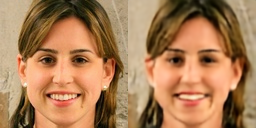
\includegraphics[width=0.24\textwidth]{LatentDiffusion/vae-samples/vae8/sample_0_0.png}%
  \hfill
  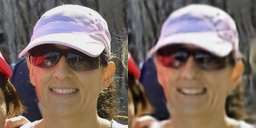
\includegraphics[width=0.24\textwidth]{LatentDiffusion/vae-samples/vae8/sample_0_1.png}%
  \hfill
  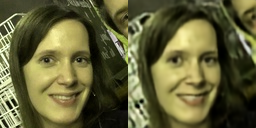
\includegraphics[width=0.24\textwidth]{LatentDiffusion/vae-samples/vae8/sample_0_2.png}%
  \hfill
  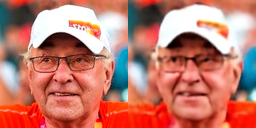
\includegraphics[width=0.24\textwidth]{LatentDiffusion/vae-samples/vae8/sample_0_3.png}
	
	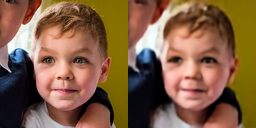
\includegraphics[width=0.24\textwidth]{LatentDiffusion/vae-samples/vae8/sample_0_4.png}%
  \hfill
  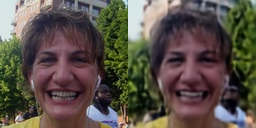
\includegraphics[width=0.24\textwidth]{LatentDiffusion/vae-samples/vae8/sample_0_5.png}%
  \hfill
  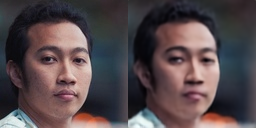
\includegraphics[width=0.24\textwidth]{LatentDiffusion/vae-samples/vae8/sample_0_6.png}%
  \hfill
  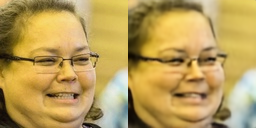
\includegraphics[width=0.24\textwidth]{LatentDiffusion/vae-samples/vae8/sample_0_7.png}
\end{figure}



\begin{figure}[h]
	\caption{Input and Reconstructed Images with Latent Size 32 $\beta$}
	\label{fig:samples}
	\centering
	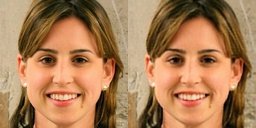
\includegraphics[width=0.24\textwidth]{LatentDiffusion/vae-samples/vae32/sample_0_0.png}%
	\hfill
	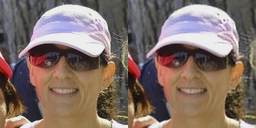
\includegraphics[width=0.24\textwidth]{LatentDiffusion/vae-samples/vae32/sample_0_1.png}%
	\hfill
	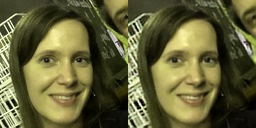
\includegraphics[width=0.24\textwidth]{LatentDiffusion/vae-samples/vae32/sample_0_2.png}%
	\hfill
	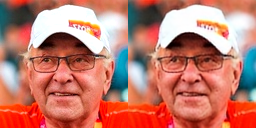
\includegraphics[width=0.24\textwidth]{LatentDiffusion/vae-samples/vae32/sample_0_3.png}

	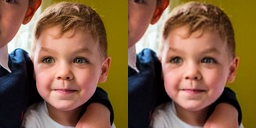
\includegraphics[width=0.24\textwidth]{LatentDiffusion/vae-samples/vae32/sample_0_4.png}%
	\hfill
	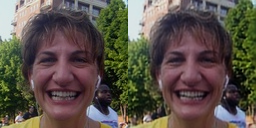
\includegraphics[width=0.24\textwidth]{LatentDiffusion/vae-samples/vae32/sample_0_5.png}%
	\hfill
	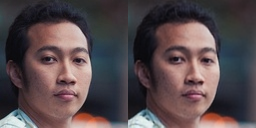
\includegraphics[width=0.24\textwidth]{LatentDiffusion/vae-samples/vae32/sample_0_6.png}%
	\hfill
	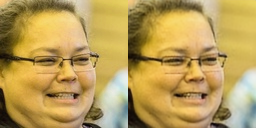
\includegraphics[width=0.24\textwidth]{LatentDiffusion/vae-samples/vae32/sample_0_7.png}
\end{figure}

Increasing the latent size led to an increase in the reconstruction quality. It might lead to a loss of continuity which is hard to quanitfy.

\subsection{(b)}

\begin{figure}[h]
	\caption{Plot of Alphas and Betas}
	\label{fig:alphasbetas}
	\centering
	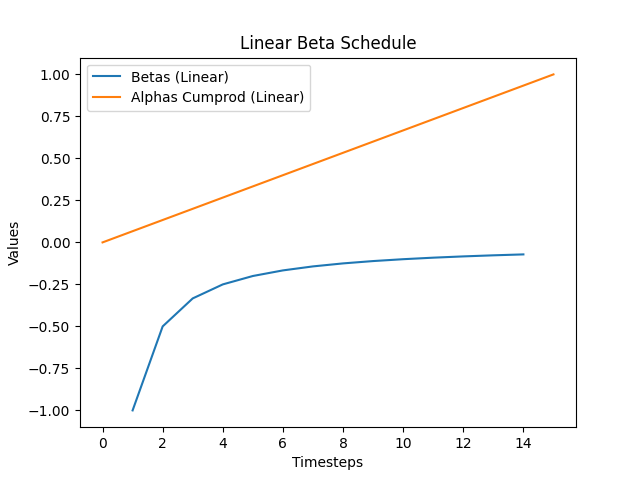
\includegraphics[width=0.45\textwidth]{report/alphas_betas_linear.png}%
	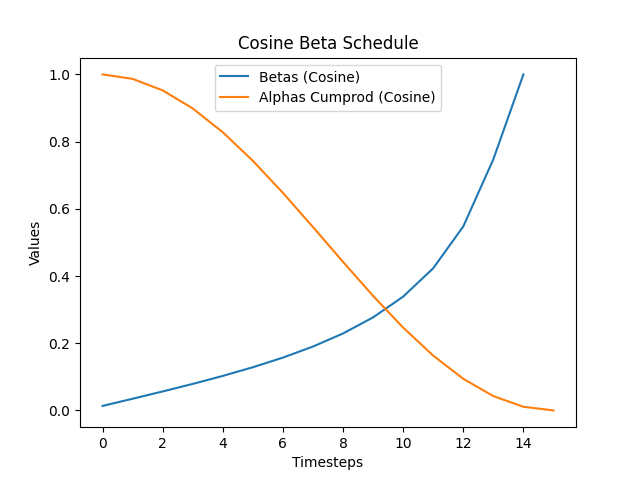
\includegraphics[width=0.45\textwidth]{report/alphas_betas_cosine.png}%
\end{figure}

\vspace{-10pt}


\begin{figure}[h]
	\caption{Linear noise schedule}
	\label{fig:inprec1}
	\centering
	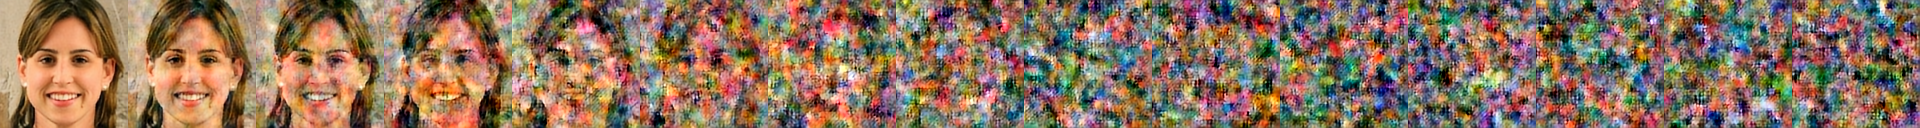
\includegraphics[width=1\textwidth]{report/sample_noised_linear.png}%
\end{figure}
\newpage

\begin{figure}[h]
	\caption{Cosine noise schedule}
	\label{fig:inprec2}
	\centering
	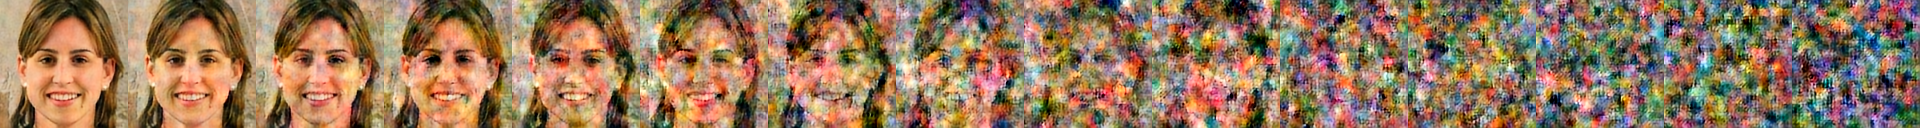
\includegraphics[width=1\textwidth]{report/sample_noised_cosine.png}%
\end{figure}
Linear noise schedule adds noise at a constant rate during the forward diffusion process. This results in more stable training and smoother denoising. The denoiser learns to handle predictable noise. It might not capture more complex noise patterns compared to a cosine schedule.

A cosine noise schedule introduces noise more gradually at first, then increases it rapidly later on, potentially making it harder for the model to learn to denoise in later stages but allowing for more nuanced noise handling early in training.

\section{Exercise 2}
See code for implementation.

\newpage
\begin{figure}[h]
	\caption{Training loss of denoiser}
	\label{fig:inprec2}
	\centering
	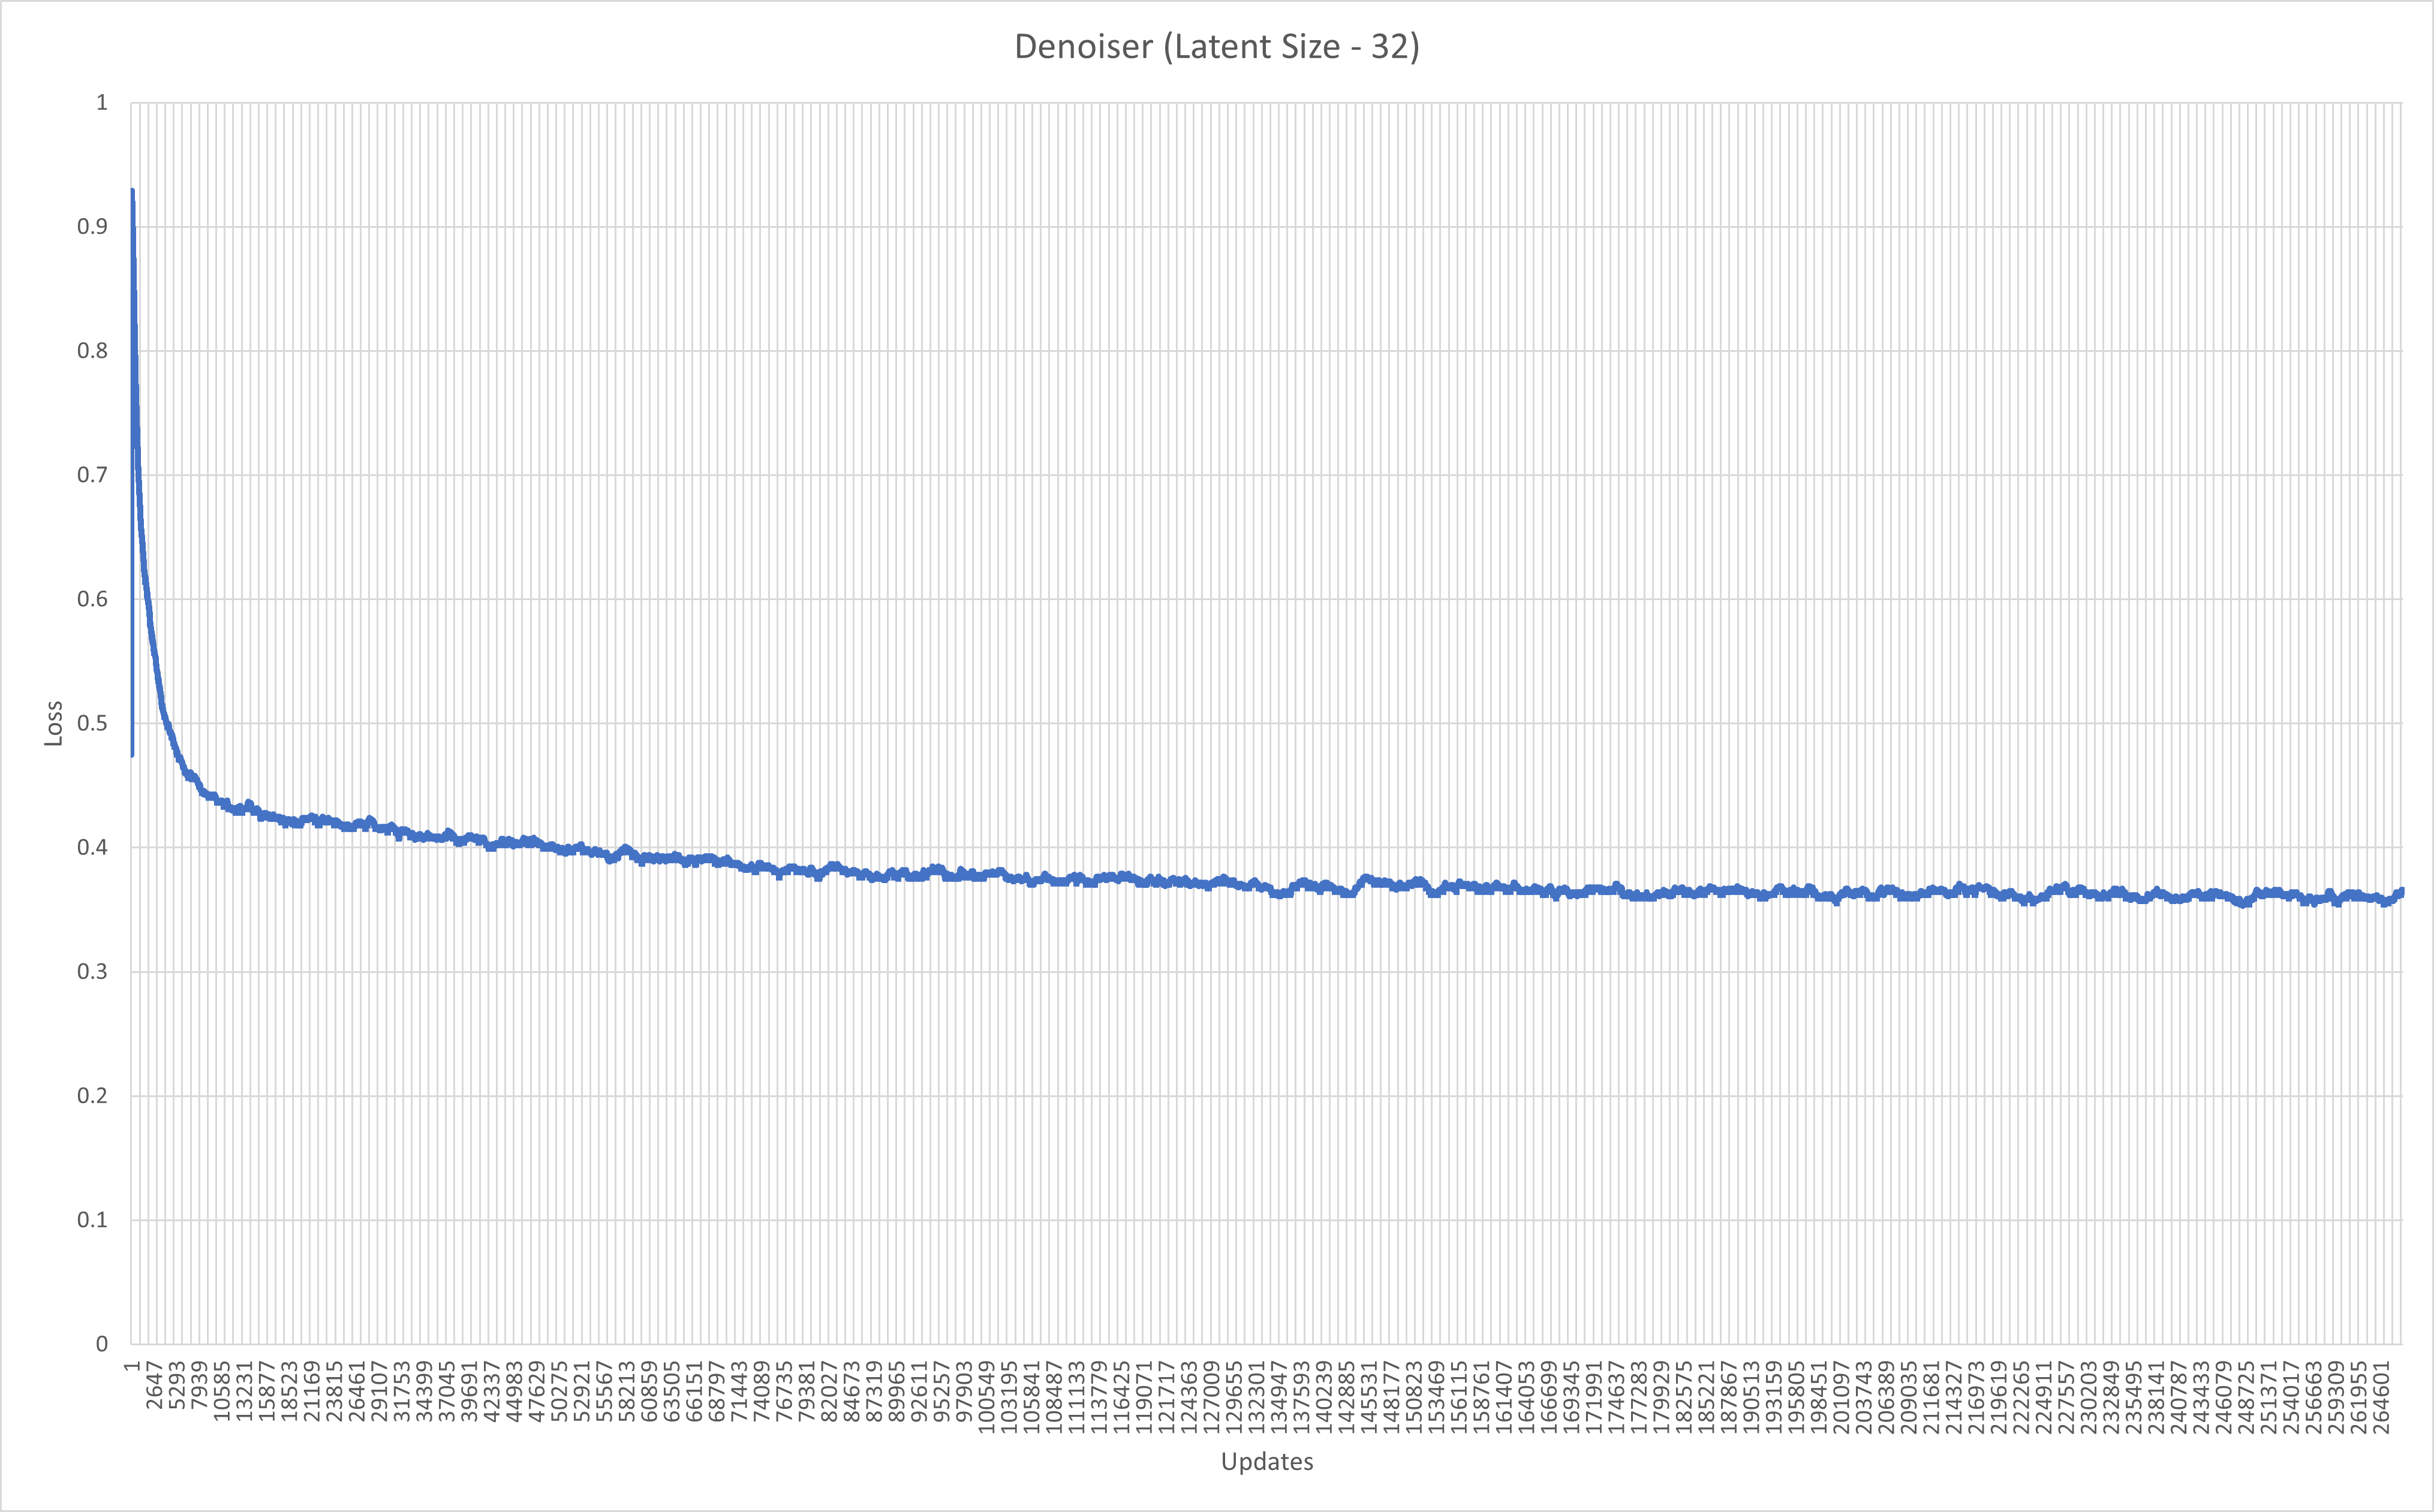
\includegraphics[width=1\textwidth]{report/trainlossDenoiser32.png}%
\end{figure}

The loss converges to around 0.34 early in the training and then becomes unstable.
We tried with Latent Size-8(default config) and Size-32, adjusting the batch size and learning rate for them respectively and both seem to converge to around the same loss. We weren't able to optimize the hyperparameters as the denoiser didn't produce meaningful results for either latent size.

\section{Exercise 3}

\newpage
\begin{figure}[h]
	\caption{DDPM Samples :')}
	\label{fig:ddpmsamples}
	\centering
	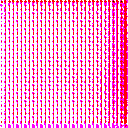
\includegraphics[width=0.24\textwidth]{LatentDiffusion/diffusion-samples/ddpm32/sample_1.png}%
	\hfill
	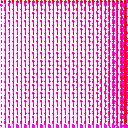
\includegraphics[width=0.24\textwidth]{LatentDiffusion/diffusion-samples/ddpm32/sample_2.png}%
	\hfill
	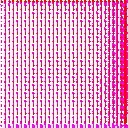
\includegraphics[width=0.24\textwidth]{LatentDiffusion/diffusion-samples/ddpm32/sample_3.png}
	\hfill
	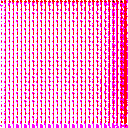
\includegraphics[width=0.24\textwidth]{LatentDiffusion/diffusion-samples/ddpm32/sample_4.png}%
	\hfill
	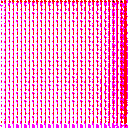
\includegraphics[width=0.24\textwidth]{LatentDiffusion/diffusion-samples/ddpm32/sample_5.png}%
	\hfill
	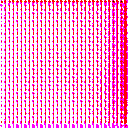
\includegraphics[width=0.24\textwidth]{LatentDiffusion/diffusion-samples/ddpm32/sample_6.png}%
	\hfill
	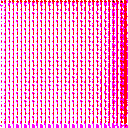
\includegraphics[width=0.24\textwidth]{LatentDiffusion/diffusion-samples/ddpm32/sample_7.png}
	\hfill
	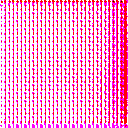
\includegraphics[width=0.24\textwidth]{LatentDiffusion/diffusion-samples/ddpm32/sample_8.png}%
\end{figure}

\begin{figure}[h]
	\caption{Reverse diffusion process of sample 1}
	\label{fig:ddpmcollage}
	\centering
	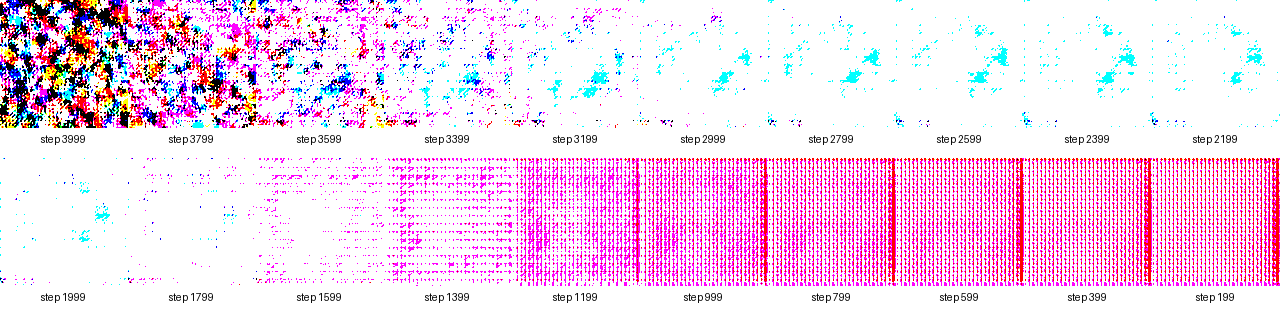
\includegraphics[width=1\textwidth]{LatentDiffusion/diffusion-samples/collage.png}%
\end{figure}

The generated images unfortunately do not improve but converge to an incorrect output which optimizes the loss.

\section{Exercise 4}
\newpage
\begin{figure}[h]
	\caption{Derivation}
	\label{fig:derivation}
	\centering
	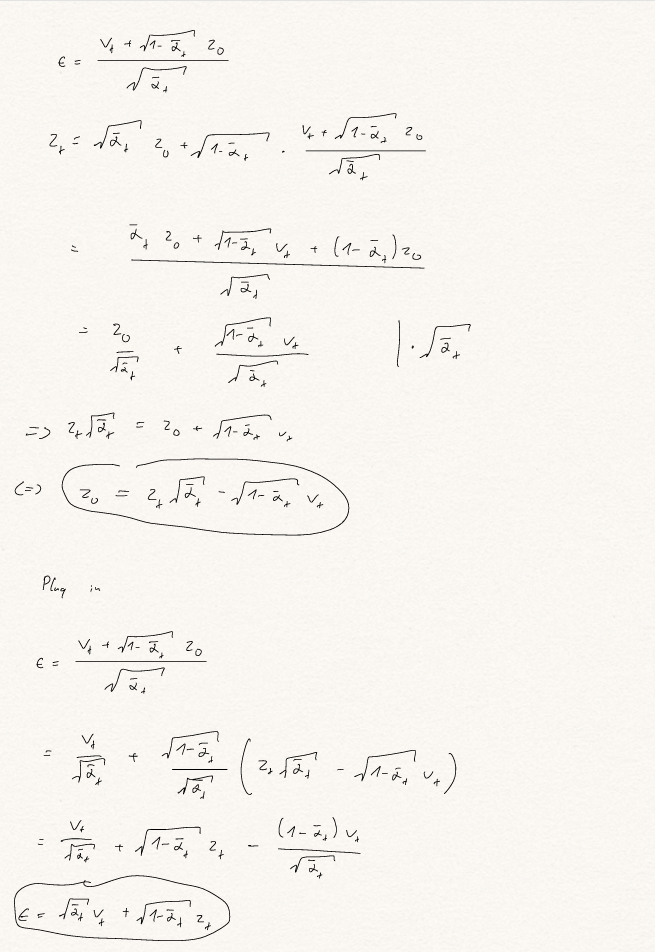
\includegraphics[width=1\textwidth]{report/derivation.png}%
	\end{figure}

\newpage
\begin{figure}[h]
	\caption{DDIM Samples :')}
	\label{fig:ddimsamples}
	\centering
	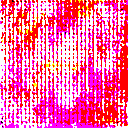
\includegraphics[width=0.24\textwidth]{LatentDiffusion/diffusion-samples/ddim32/sample_1.png}%
	\hfill
	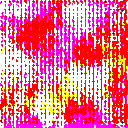
\includegraphics[width=0.24\textwidth]{LatentDiffusion/diffusion-samples/ddim32/sample_2.png}%
	\hfill
	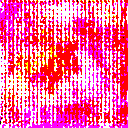
\includegraphics[width=0.24\textwidth]{LatentDiffusion/diffusion-samples/ddim32/sample_3.png}
	\hfill
	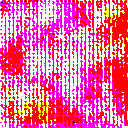
\includegraphics[width=0.24\textwidth]{LatentDiffusion/diffusion-samples/ddim32/sample_4.png}%
	\hfill
	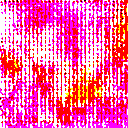
\includegraphics[width=0.24\textwidth]{LatentDiffusion/diffusion-samples/ddim32/sample_5.png}%
	\hfill
	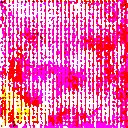
\includegraphics[width=0.24\textwidth]{LatentDiffusion/diffusion-samples/ddim32/sample_6.png}%
	\hfill
	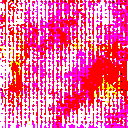
\includegraphics[width=0.24\textwidth]{LatentDiffusion/diffusion-samples/ddim32/sample_7.png}
	\hfill
	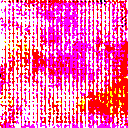
\includegraphics[width=0.24\textwidth]{LatentDiffusion/diffusion-samples/ddim32/sample_8.png}%
\end{figure}
\end{document}

